\documentclass[12pt]{article}
\usepackage{graphicx}
\usepackage{attachfile}
\usepackage{float}
\graphicspath{ {./images/} }

\title{Work at the Mdls Lab Documentation}
\author{Mobbili Leonardo}

\begin{document}

\maketitle

\section{Analyze the dataset}
The first step I needed to do was to have a complete description
of the crucial columns of the dataset that I needed to work on.
This is important to understand the data and to be able to
analyze the dataset. 
I then loaded the data into a jupyter notebook and using pandas 
and matplotilib I did basic statistics and plotting to 
try to understand the data better.
After that I filtered the dataset to keep only the columns
that were relevant for my analysis and created a new Excel file
to store the filtered data.
\pagebreak
\subsection{Plotting and statistics}
The first statistic that I did was to calculate the mean and 
plot the age distribution of the patients in the dataset.
\begin{figure}[H]
  \centering
  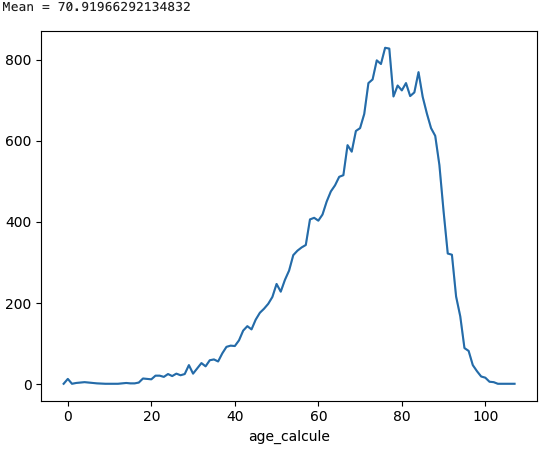
\includegraphics[width=0.7\linewidth]{ageDistribution.png}
  \caption{Age distribution plot}
  \label{fig:dataset-plot}
\end{figure}
\pagebreak
\noindent I then procided to calculate for each column how many 
missing values there were. (see attached file)
\attachfile[description=attached file,icon=Paperclip,]{/Users/lm287091/Documents/Work-Docs/countNull.xlsx}.

\noindent I calculated the sex distribution of the patients in the dataset
and plotted it as a pie chart.
  \begin{figure}[H]
    \centering
    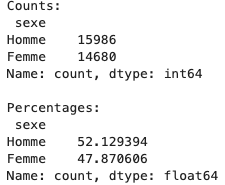
\includegraphics[width=0.5\linewidth]{sexDIstribution.png}
    \caption{Sex distribution counts and percentages}
    \label{fig:dataset-plot2}
  \end{figure}
  \begin{figure}[H]
    \centering
    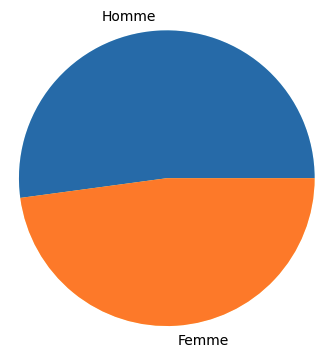
\includegraphics[width=0.5\linewidth]{sexDistributionPlot.png}
    \caption{Sex distribution plot}
    \label{fig:dataset-plot3}
  \end{figure}
\pagebreak
\noindent The next step was to calculate the distribution of the
patients between the different centers involved in the study.
The full distribution is shown in the attached file. (see attached file)
\attachfile[description=attached file,icon=Paperclip,]{/Users/lm287091/Documents/Work-Docs/centersCounts.xlsx}.

\noindent I also plotted the distribution of the patients 
between the different centers as a pie chart leaving out the centers with
less than 100 patients.
\begin{figure}[H]
  \centering
  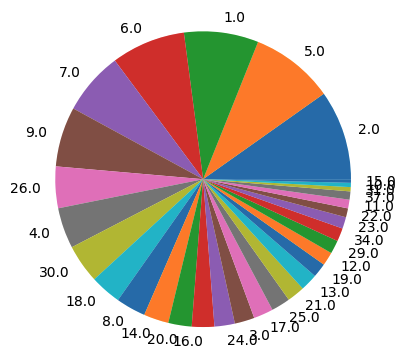
\includegraphics[width=0.8\linewidth]{centersDistributionPlot.png}
  \caption{Centers distribution plot}
  \label{fig:dataset-plot4}
\end{figure}
\pagebreak
\noindent Another interesting statistic was to calculate the number
of patients that recieved intravenous thrombolysis.
\begin{figure}[H]
  \centering
  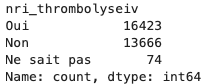
\includegraphics[width=0.5\linewidth]{numThrombo.png}
  \caption{Thrombolysis distribution statistic}
  \label{fig:dataset-plot5}
\end{figure}
\begin{figure}[H]
  \centering
  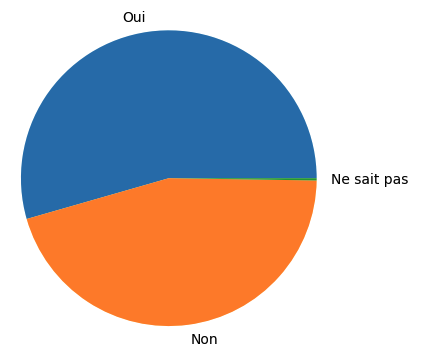
\includegraphics[width=0.7\linewidth]{numThromboPlot.png}
  \caption{Thrombolysis distribution plot}
  \label{fig:dataset-plot6}
\end{figure}
\pagebreak
\noindent This next statisctic show the number of patients for each 
grade of MRS at 3 months (Lower is better).
\begin{figure}[H]
  \centering
  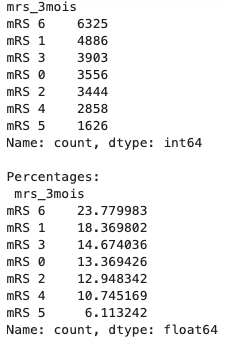
\includegraphics[width=0.4\linewidth]{mrs3Months.png}
  \caption{MRS at 3 months distribution statistic}
  \label{fig:dataset-plot7}
\end{figure}
\begin{figure}[H]
  \centering
  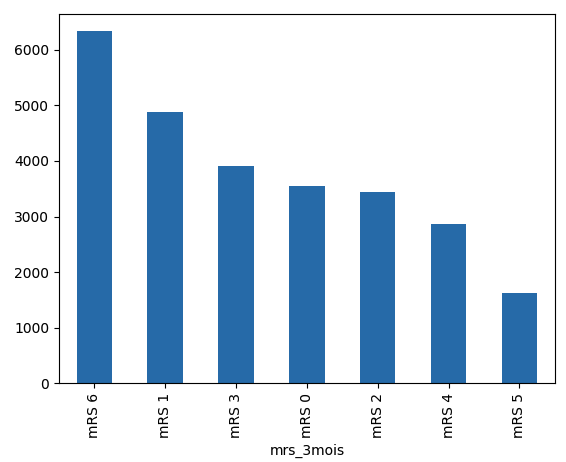
\includegraphics[width=0.6\linewidth]{mrs3MonthsPlot.png}
  \caption{MRS at 3 months distribution plot}
  \label{fig:dataset-plot8}
\end{figure}
\pagebreak
\noindent One of the most crucial statistic is the aspectj0

\noindent (Brain area not affected \textrightarrow 10 = perfect, 0 = entire brain affected)
\end{document}